\documentclass{llncs}
\usepackage{graphicx}
\usepackage{amsmath,amssymb}
\usepackage[english]{babel}
\usepackage[utf8]{inputenc}
\usepackage[ruled,vlined]{algorithm2e}
\usepackage{url}
\usepackage{float}%figure environment
\usepackage{multirow}
\usepackage{booktabs}
\usepackage{todonotes}
\usepackage{booktabs}
\usepackage{mdframed}
\usepackage{graphicx}
\usepackage{wrapfig}



\begin{document}
\title{Combining Linked Data and Statistical Information Retrieval} 
\subtitle{Next Generation Information Systems}
\author{
Ricardo Usbeck
}

\institute{
University of Leipzig, Germany\\
\email{\{usbeck$|$ngonga\}@informatik.uni-leipzig.de}\\
R\,\&\,D, Unister~GmbH, Leipzig, Germany
}

\maketitle
Advisors: Axel-Cyrille {Ngonga Ngomo}, Andreas Both and Sören Auer

\begin{abstract}
Being a part of the \emph{Information Age}, users are challenged with a tremendously growing amount of Web data which generates a need for more sophisticated information retrieval systems.
The \emph{Semantic Web} provides necessary procedures to augment the highly unstructured Web with suitable metadata in order to leverage search quality and user experience.
In this article, we will outline an approach for creating a web-scale, precise and efficient information system capable of understanding keyword, entity and natural language queries.
By using Semantic Web methods and \emph{Linked Data} the doctoral work will present how the underlying knowledge is created and elaborated searches can be performed on top.
\end{abstract}
\textbf{Keywords:} Search, NLP, Question Answering, Ranking

\section{Introduction}

In the last couple of years, the way search is perceived by end users as well as industrial agents changed dramatically.
Recently, new semantic search algorithms\footnote{\url{http://searchengineland.com/google-hummingbird-172816}} spread which account not only for keywords but for semantic entities, relations, personalized information and many more.
In analogy, future developments in everyday and business search engines need to unlock the power of semantic technologies.

Linked Data is the Semantic Web methodology for publishing data based on W3C standards such as RDF~\cite{RDF-PRIMER}, URI and HTTP in order to provide linkable, valuable content.
Whether provided by a SPARQL~\cite{SPARQL} endpoint or embedded in a Web page via RDFa~\cite{RDFA}, Linked Data is a key technology to master the upcoming information flood.
Since 2007, the Linked Open Data (LOD) Cloud gathered more than 300 datasets also known as \emph{knowledge bases} comprising over 31 billion triples\footnote{\url{http://lod-cloud.net/state/}}.
Amongst others it consists of agricultural, musical, medical and geographical facts, the LOD Cloud is the largest linked encyclopaedic knowledge base known to mankind.

Using the Semantic Web is expected to drive innovation in data integration and analysis software within companies.
Moreover, end users anticipate more sophisticated search engines that truly understand the underlying information need.
Therefore, combining scientifically sound information retrieval methods with static and dynamic Web data as well as Linked Data will leverage information insight already in the short term.
For example, fundamental scientific work has been done in the Linked Open Data~\cite{lod2} project.
However, there is no information retrieval framework which is able to convert the scientific knowledge into a holistic Semantic Web-based search engine.

In Section~\ref{relatedWork}, the state of the art in the areas of information retrieval and Linked Data-based search and ranking algorithms is presented. 
The problems tackled in this thesis and its contributions are described in Section~\ref{contributions}.
Section~\ref{approaches} presents the already available approaches \emph{AGDISTIS}~\cite{AGDISTIS}, which is a named entity extraction framework for unstructured Web pages, and \emph{REX}~\cite{REX}, a relation extraction approach for templated websites. 
Furthermore, first steps towards an auto-completion functionality are pointed out and plans on further research regarding search and ranking algorithms are presented. 
Section~\ref{conclusion} concludes with an outlook on the future research agenda.

\section{State of the Art}\label{relatedWork}
\begin{itemize}
\item[(1)]\emph{Information Extraction.} This field can be considered as comprising three main sub-fields: named entity recognition (NER), named entity disambiguation (NED) and relation extraction (RE).
NER is the task of identifying entities in an input text while NED is focused on pre-identified  named entities and their disambiguation towards a certain knowledge base using various methods.
RE is the task of finding connections between entities based on a given context.
In this thesis, we restrict the identifiable entity classes to 'persons', 'locations' and 'organizations' using FOX~\cite{FOX} as well-known NER framework.

In the following, several NED approaches for \emph{unstructured texts} are introduced.
A framework for annotating and disambiguating Semantic Web resources in unstructured texts is DBpedia Spotlight~\cite{spotlight}.
Contrary to other tools, Spotlight is able to disambiguate against all classes of the DBpedia ontology.
Another algorithm is AIDA which uses the YAGO2\footnote{\url{http://www.mpi-inf.mpg.de/yago-naga/yago/}} Linked Data knowledge base using sophisticated sub-graph matching algorithms. 
Furthermore, the approach disambiguates w.r.t.~similarity of contexts, prominence of entities and context windows.
Unfortunately, the approaches presented so far are either not efficient enough (i.e. runtime lacks~\cite{cornolti}) to handle web-scale data or do not deliver the expected extraction quality based on specific Linked Data sources~\cite{AGDISTIS}.
Recently, Cornolti et al.~\cite{cornolti} presented a framework for benchmarking NED approaches.
The authors compared six existing approaches against five well-known datasets on different tasks and with different measures. 

Information Extraction from \emph{templated web-sites} is mainly related to the field of wrapper induction. 
Early approaches to learning web wrappers were mostly supervised (e.g.,~\cite{Hogue:2005:TAU:1060745.1060762,flesca2004web}). 
Recently, Crescenzi et al~\cite{Crescenzi2013} described a supervised framework that is able to profit from crowd-provided training data. 
The learning algorithm controls the cost of the crowdsourcing campaign w.r.t. quality of the output wrapper.
However, these novel approaches miss the opportunities related to existence of Linked Data, and the semantic consistency of the extracted data is out of their scope of interest.

In order to accomplish the vision of the Semantic Web, Gentile et al.~\cite{Gentile2013} presents an approach for learning web wrappers that exploit Linked Data as a training data source for their wrapper induction framework. 
However, the process they adopt consists of a variety of manual steps and is thus very time consuming.


\item[(2)]
\emph{Search Query Support.}Auer et al.~\cite{conjunctiveQueries} describe a method to enrich search queries via a conjunctive extension based on the underlying semantic ontology. This approach is able to retrieve entities and documents provided only with a description instead of a search query. 
This leads to results without an overlap of keywords between query and document.

Besides keyword-based search queries, some search engines also understand natural language questions. 
Question answering is more difficult than keyword-based searches since retrieval algorithms need to understand complex grammatical constructs.
Unger et al.~\cite{template} present a manually curated, template-based approach to match a question against a specific SPARQL query. 
They combine natural language processing (NLP) capabilities with Linked Data which leads to good benchmark results w.r.t. the question answering on Linked Data benchmark (QALD)\footnote{\url{http://greententacle.techfak.uni-bielefeld.de/~cunger/qald}}.

\item[(3)]
\emph{Information Retrieval/Hybrid Search.}Popular search engines like Google or Yahoo! have answered search requests based on keyword queries for a long time. 
For a retrospective of existing information retrieval methods the interested reader may refer to standard literature~\cite{IRBook}.
However, the development of Semantic Web technologies lead to search engines being more conversational than traditional keyword-based engines~\cite{googleKeynote}.
%Below, we introduce information retrieval algorithms based on keyword search requests.
%First of all, the \emph{boolean retrieval} based on boolean logic and set theory has been explored.
%A keyword-based search query $q$ is considered as a formula $f$ out of the sequence of terms $t_1,\dots,t_n$ from q and logical operates like $\wedge,\vee,\neg$. 
%A document $d = \{ t_i,\dots,t_j \}$ is relevant iff it satisfies $f$.
%Another approach is the \emph{vector space model}, where a document is handled as a vector over its terms $d'=(d_1,\dots,d_V)$ w.r.t. to a certain vocabulary $V$.
%Therefore, the relevance of a document can be defined as a vector similarity, e.g., cosine distance~\cite{FrakesB92}. 

Apart from those document- and keyword-centric approaches, the Linked Data movement has developed diverse strategies to leverage the advantages of semantic knowledge.
Based on the underlying semantic structure of Linked Data, He et al.~\cite{graphBasedSemanticIndexing} developed an approach that transforms search queries to semantic graphs and tries to match those against the Linked Data graphs of the underlying dataset.

Furthermore, \url{http://swoogle.umbc.edu} represents a first prototype of a semantic search engine.  	
Ding et al.~\cite{Ding05findingand} described the different search strategies to find instances via, e.g., term, document or ontology searches.
Since this application was updated in 2007 for the last time and only consists of a comparably small corpus of documents and Linked Data, it cannot be considered as a web-scale approach.

\url{http://sindice.com/}~\cite{sindice} is a more recent approach that scans the Semantic Web in order to build a semantic web index that is searchable and queryable via SPARQL.
Unfortunately, the underlying database does not comprise full-text information and thus cannot answer a broad range of queries.

\item[(4)]
\emph{Ranking}

The procedures and algorithms described before are capable of delivering an unordered set of search results to the user. 
However, the increasing number of documents available on the Web leads to a tremendous growth of search result sets. 
Following Smyth et al.~\cite{Smyth05alive-user}, most users tend to look only at the first few results.
To aid finding relevant information within the first few places, ranking algorithms need to be deployed.

Well-known representatives for Web document ranking algorithms are the Hypertext-Induced Topic Search (HITS) algorithm~\cite{HITS} and \mbox{PageRank~\cite{PageRank}}. Both calculate the relevance of a search result based on the Web link graph and are also very scalable algorithms.

Already in 2002, Mayfield et al.~\cite{MF03,Shah:2002} described a first approach combining information retrieval with semantic inference mechanism. Furthermore, they present an algorithm which ranks Semantic Web entities with regard to trust information.

Moreover, an extension to the PageRank algorithm using Linked Data knowledge has been described by Julia Stoyanovich~\cite{Stoyanovich}. Extracting semantic knowledge from a Web document and combining this with an underlying ontology has shown to improve ranking quality. Unfortunately, this version of the algorithm is not able to scale on Web data. 

Furthermore, ReConRank~\cite{reconrank} is a highly efficient algorithm based on the \mbox{PageRank} algorithm. 
It considers provenance information while ranking, leading to more trustworthy result lists. 
This algorithm is based on semantic sub-graphs whose size influences efficiency and precision of results. 

The ranking algorithms described so far are independent of the underlying query which can steer those towards a loss of information.
Gupta et al.~\cite{gupta} introduced an approach that enriches the query based on Linked Data in order to find, e.g., polysemes and synonyms. 
Afterwards, the ranking works on a context-ordered index retrieving an initial sorting of the documents, which are finally sorted according to their similarity to the query.

Moreover, xhRank~\cite{xhRank} proves that a combination of semantic information from a Linked Data graph can lead to an improved ranking. The position, morphological features and structure of an entity within a query are used to reorder certain documents from the search result list.

Past attempts combining Linked Data and information retrieval techniques suffer from either performance leaks and high quality results with respect to Web-scale datasets or a missing holistic concept that is able to bring search technology to the next level.

\end{itemize}
\section{Problem Statement and Contributions}\label{contributions}

The aim of this doctoral work is an information system/search engine framework that will address the following working domains: 
\begin{itemize}
\item[(1)]Initially, the proposed system needs to link crawled Web data with Semantic Web knowledge.
This task can be performed by NER, NED and RE algorithms. 
Therefore, two types of Web pages need be distinguished: templated sites like actor pages from \url{http://www.imdb.com/} and unstructured Web pages like news articles from \url{http://www.nytimes.com/}.
In this thesis, two \emph{Information Extraction} approaches have been developed, which are described in Section~\ref{approaches}.
\item[(2)]After the data is provided, the user has to be enabled to search it. 
An effective way to do so is to provide the user with a input field-like interface they are used to. 
As the user begins typing into the search input field the framework should present different search query suggestions.
This \emph{auto-completion} does not only speed up searching but also teaches the user which kind of queries the search engine framework understands. 
Moreover, this can lead to a reeducation of users' search behavior from short keyword-based searches to longer natural language queries or even real search questions.
An auto-completion approach which \emph{supports the query generation} will be developed in the next stage of the PhD work using linked knowledge.

\item[(3)]The search functionality to be developed in this thesis is going to be \emph{hybrid}, i.e., simultaneously performing a full-text,e.g., Lucene-based\footnote{\url{http://lucene.apache.org/core/}}, and an entity search. 
Different entity search algorithms need to be developed based on the significantly different data structures and problems arising from them. 
While full-text search is a well-studied field, as shown in Section~\ref{relatedWork}, entity search on Linked Data has only been in the focus of research for about 10 years.
A hybrid search engine is currently under development and will be evaluated against the recently published QALD-4 benchmark.

\item[(4)]Finally, when appropriate Web pages and Semantic Web entities have been found, the user wants them to be presented according to their relevance.
\emph{Ranking} algorithms aim to reorder result list with respect to one or more sorting criteria.
Scientifically sound methods for classical information retrieval are already present and the most important ones can be found in Section~\ref{relatedWork}.
However, principles creating a combined ranking of full-text and semantic search results need to be investigated within this doctoral thesis.
Therefore, we aim at creating an machine learning-based interweaving of several well-known ranking algorithms.
\end{itemize}

Combining the advantages of information retrieval methods and Linked Data technologies will overcome the information flood problem. 
The union of highly scalable retrieval algorithms and effective rankings is able to increase the users search experience.
A formalisation of the approach is currently in progress.

\section{Research Approach and Initial Results}\label{approaches}

Central to this PhD work is to answer \emph{how a search engine can benefit from the Linked Data paradigm?}
Diverse technologies like RDFa, micro-data and HTML5 semantic annotations have been introduced to enrich Web data for a better user experience and machine interoperability.
However, to the best of our knowledge there is no information retrieval architecture that uses the advantages of this technology holistically. 
Moreover, some search pipeline steps for the Web of Data need to be revised in order to perform efficient and effective searches.

To meet this obstacle, the presented thesis introduces a pipeline architecture for a Linked Data-based search engine, as depicted in Figure~\ref{overview}.

\begin{figure*}[h!tb]
    \centering
        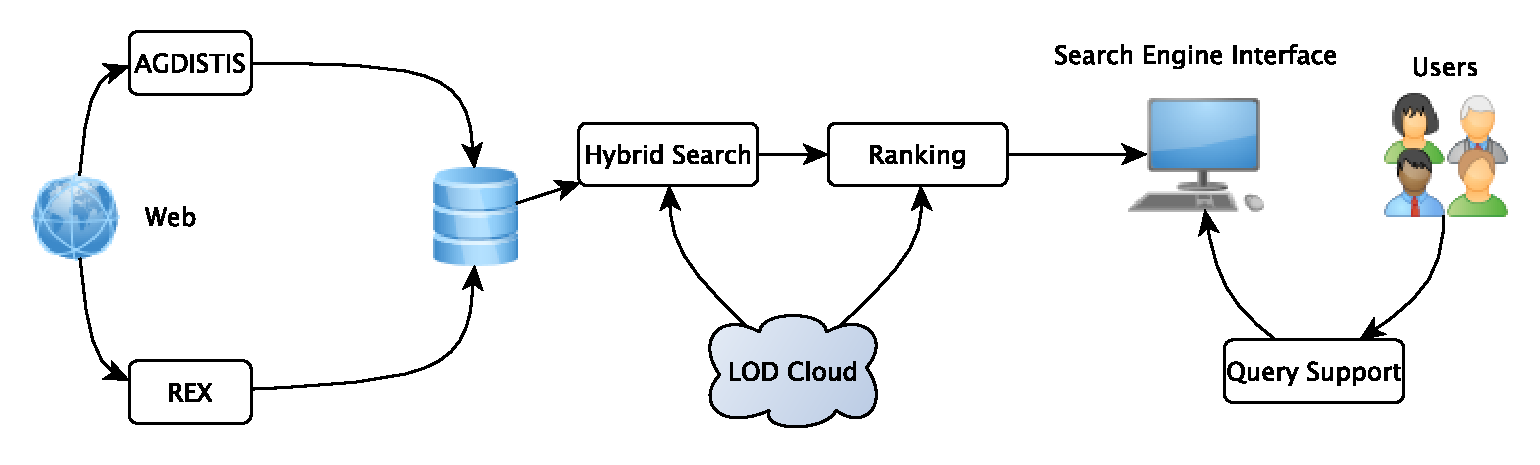
\includegraphics[width=\linewidth]{overview.pdf}
    \caption{Overview of the proposed information system architecture.}
    \label{overview}
\end{figure*}

The starting point of the proposed architecture is a two-fold data acquisition strategy based on a highly efficient, state-of-the-art industry Web crawler provided by our research partner \emph{Unister GmbH}.  

First, \emph{unstructured Web pages} from the crawled dataset, e.g., provided texts from news portals or agencies, are annotated by a standard NER algorithm~\cite{stanford} followed by a novel NED approach AGDISTIS~\cite{AGDISTIS}.
This NED approach has been developed to support arbitrary Linked Data knowledge bases to ensure future developments.
Moreover, AGDISTIS uses several NLP techniques to identify a set of candidate entities and identifies the correct with the help of the graph-based HITS algorithm. % and the resulting authority scores.
To prove the quality of AGDISTIS' results several corpora have been generated, evaluated and published. 
These corpora, called $N^3$~\cite{n3}, use the state-of-the-art serialization format \emph{NIF}~\cite{NIF} following the ``eating our own dogfood'' paradigm inherent to the Semantic Web community. 
$N^3$ are expected to form a novel gold standard in the areas of semantic named entity recognition and disambiguation.
Using $N^3$ and other well-known datasets, AGDISTIS has been proven to outperform the state-of-the-art algorithm AIDA~\cite{AIDA} by up to $16\%$ F-measure.
In the future, AGDISTIS will be evaluated against the framework of Cornolti et al.~\cite{cornolti} to provide a more comprehensive evaluation. 

Second, \emph{templated Web pages}, e.g., \url{http://www.imdb.com}, have been identified as another important source for answering user searches.
Therefore, REX~\cite{REX} has been developed during the early stage of this PhD work.
It is a web-scale semantic relation extraction framework capable to identify known as well as novel relations on Web pages creating RDF out of them.
REX combines a well-known wrapper induction technique~\cite{Crescenzi2013} for extracting XPath expressions, AGDISTIS as its NED algorithm and a consistency checker for the extracted relations based on ad-hoc generated schemas.
It has been shown that REX is able to generate new Linked Data triples with a precision of above $75\%$~\cite{REX}.

The resulting data from both pre-processing steps will serve as the underlying dataset for future research steps together with knowledge from the LOD Cloud.

Concerning the users' need for exploring the data space, %by enabling searches via keywords, natural language or even questions 
the next step is to \emph{support the formulation of queries}.
A huge potential within classical search engines is contained in inexact search queries, e.g., in terms of given a description only or a question.
Standard search engine methodologies fail at this point due to not being able to match keyword queries. 
In this thesis, we will support query formulation by providing on-the-fly recommended queries based on the real-time user input.
It is planned to use Linked Data such as \emph{BabelNet}\footnote{\url{http://babelnet.org/}} to find polysemes and synonyms within a query and thus enhancing the understanding of what the users actually mean.
Furthermore, three different standard approaches as well as a Linked Data-based grammar will be compared and evaluated against each other.
Another by-product of an according auto-completion approach is to teach the user which queries a search engine understands.

The research field of information retrieval/search and ranking has so far only been analysed theoretically within this doctoral work. 
In this thesis, a hybrid search engine is going to be implemented, i.e., an engine comprising a full-text information retrieval system enhanced by extracted Linked Data and a stake of LOD Cloud-based entity search.
Especially, the keyword-based search engine \emph{SINA}~\cite{SINA} will be a starting point for further research. 

With respect to ranking algorithms, this PhD work focuses on two different research plans.
At first, a semantic extension of graph-based authority calculating algorithms will be investigated. 
Therefore, a master thesis has been looked after which analysed a context-driven enhancement of Stoyanovich's work~\cite{Stoyanovich}.
Initial results show an improvement compared to the baseline using the plain PageRank algorithm.
In parallel, an ensemble learning approach of Semantic Web-based ranking algorithms will be evaluated.

To summarize, the aforementioned steps will help building an integrated information system leveraging search engine performance using Linked Data.
Additionally--due to strong industry needs--this framework is going to be used in a real-life environment with web-scale amounts of users.
Finally, most of the source code will be published as open source and can be downloaded via the projects homepage\footnote{\url{http://aksw.org/RicardoUsbeck}}.

\section{Evaluation Plan and Conclusion}\label{conclusion}
This PhD work is dimensioned for three years. 
After intense literature reviews in the beginning of the first year the need for annotated Web data has been identified.
As a logical consequence, the development of AGDISTIS and REX had been finished by the end of the first year. 
Alongside, a gold standard ($N^3$) has been created to be able to evaluate the approaches mentioned above.

The second year will be used for developing and assessing the corresponding search and ranking procedures. 
To measure the quality of the \emph{auto-completion} technology, we assess different real-world query logs from our industry partner.
Thereby, we analyze how much characters are need to understand the query correct.
Additionally, we focus on the efficiency of the system in terms of milliseconds to react on a pressed key.

Considering the ranking evaluation, we will use standard precision, recall and f-measures as well as rank comparision measures, e.g., mean reciprocal rank. 
The underlying data is provided by the industry partner through human rater assessments and several comparisons to real-life search engines, e.g., Google or Wolfram Alpha.

Afterwards, the combined pipeline itself will be evaluated in a qualitative study using professionals and end users.
Therefore, empirical methods like Likert-scale questionnaires and direct relevance feedback will be used.


Next to refining already submitted work and optimizing the source code to meet industrial production standards, the developed approaches and algorithms will be refined in a spiral way if unpredictable results occur.
Thereby, upcoming ideas will be interweaved with the presented schedule creating a closed loop consisting of research question, development, evaluation and new research questions.


\section*{Acknowledgements}
\begin{wrapfigure}[2]{l}{0.3\textwidth}
 \vspace{-10mm}
 
\includegraphics[width=0.3\textwidth]{esf.pdf}
\end{wrapfigure}
This work has been supported by the ESF and the Free State of Saxony.

\bibliographystyle{plain}
\bibliography{references,aksw,limes,myrefs}

\end{document}

